\chapter{奇异值分解}
特征值和特征向量只适用于方阵,对于一般的$m\times n$矩阵$A$,有没有类似的操作?

\noindent
考虑$A\tp A$和$AA\tp$,他们都是半正定的,因为$\forall x$
\[
	x\tp A\tp Ax=\norm{Ax}^2\geqslant 0,
\]
$AA\tp$同理,因此$A\tp A$和$AA\tp$都可以对角化。
\begin{definition}{奇异值}{singular value}
	$A\tp A$是半正定的,因此所有特征值$\lambda_i\geqslant 0$,矩阵$A$的奇异值(singular value)便定义为$A\tp A$特征值的平方根:$\sigma_i:=\sqrt{\lambda_i}$。

	为了后续方便,我们将所有奇异值从大到小排列:
	\[
		\sigma_1\geqslant\sigma_2\geqslant\cdots\geqslant\sigma_n\geqslant 0.
	\]
\end{definition}
由\thmref{thm:ATA inverse},$\rank(A\tp A)=\rank(A)$
\begin{theorem}{非零奇异值的数量}{number of non-zero singular value}
	$A$的非零奇异值的数量$r=\rank(A)$。
\end{theorem}
\begin{proof}
	设$\{v_1,\ldots,v_n\}$为$\RR^n$中可以把$A\tp A$对角化的一组正交归一基,$\{\lambda_1,\ldots,\lambda_n\}$为对应的特征值,则$\{Av_1,\ldots,Av_n\}$是一个正交向量集合,即$\forall i\neq j$,
	\[
		(Av_i)\tp Av_j=v_i\tp A\tp Av_j=v_i\tp(\lambda_jv_j)=0.
	\]
	假设$\lambda_1\geqslant\cdots\geqslant\lambda_r>0$是所有的正特征值,则$Av_{r+1},\ldots,Av_n=0$.
	
	%因为$\{v_1,\ldots,v_n\}$为$\RR^n$中可以把$A\tp A$对角化的正交归一基,所以
	$\forall x\in\RR^n$,$x$可以写成$x=c_1v_1+\cdots+c_nv_n$,
	%因为$\C(A)$是由$A$所有列的线性组合得到的,所以
	从而$\forall y\in\C(A)$,$y$可以被写为$\{Av_1,\ldots,Av_r\}$的线性组合:
	\[
		y=Ax=c_1Av_1+\cdots+c_rAv_r+0+\cdots+0,
	\]
	故$\{Av_1,\ldots,Av_r\}$是$\C(A)$的一组正交基,$r=\rank(A)$。
\end{proof}
\section{奇异值分解}
\begin{theorem}{奇异值分解}{singular value resolve}
	$m\times n$矩阵$A$秩为$r$,则存在一个$m\times n$的矩阵$\Sigma$ 
	\[
		\Sigma=\begin{bmatrix}
			D&0\\0&0
		\end{bmatrix},\quad D=\diag(\sigma_1,\ldots,\sigma_r).
	\]
	$m\times m$的正交矩阵$U$和$n\times n$的正交矩阵$V$,且 
	\[
		A=U\Sigma V\tp.
	\]
\end{theorem}
\begin{proof}
	直接构造出$U,\Sigma,V$。
	
	由$A\tp A$是对称矩阵,故存在一组$\RR^n$中的正交归一基$\{v_1,\ldots,v_n\}$可将$A\tp A$对角化,$\{\lambda_1,\ldots,\lambda_n\}$为对应的特征值,且$\lambda_1,\ldots,\lambda_r>0,\enspace\lambda_{r+1},\ldots,\lambda_n=0.$
	
	因为$\{v_1,\ldots,v_n\}$之间是正交的,则$\forall i\neq j$,
	\[
		(Av_i)\tp(Av_j)=v_i\tp A\tp Av_j=\lambda_jv_i\tp v_j=0.
	\]
	所以$\{Av_1,\ldots,Av_r\}$之间也是正交的,$Av_{r+1},\ldots,Av_n=0$。令
	\[
		u_i=\frac{Av_i}{\norm{Av_i}}=\frac{Av_i}{\sqrt{\lambda_i}}=\frac{Av_i}{\sigma_i},\quad i=1,\ldots,r.
	\]
	则$\{u_1,\ldots,u_r\}$是$\C(A)$的一组正交归一基。
	
	再设$\{u_{r+1},\ldots,u_m\}$是$\N(A\tp)$中的一组正交归一基,由$\N(A\tp)=\C(A)^\perp$,$\{u_1,\ldots,u_m\}$是$\RR^m$的一组正交归一基。
	
	设矩阵$U=(u_1,\ldots,u_m),\enspace V=(v_1,\ldots,v_n)$,$U$和$V$都是正交矩阵,且
	\[
		AV=(Av_1,\ldots,Av_n)=(\sigma_1u_1,\cdots,\sigma_ru_r,0,\ldots,0)=U\Sigma.
		\qedhere
	\]
\end{proof}
\begin{theorem}{}{ATA, AAT's singular value are same}
	$A\tp A$和$AA\tp$的非零特征值相同。
\end{theorem}
\begin{proof}
	假设$x_i$是$A\tp A$的特征值为$\lambda_i\neq 0$的特征向量,
	\[
		(\lambda_iI-A\tp A)x_i=0,
	\]
	左乘$A$,
	\[
		A(\lambda_iI-A\tp A)x_i=(\lambda_iI-AA\tp)(Ax_i)=0,
	\]
	又$x_i\tp A\tp Ax_i=\lambda_i x_i\tp x_i>0$,所以$Ax_i\neq 0$,所以$Ax_i$是$AA\tp$的特征值为$\lambda_i$的特征向量。
	
	同理,如果$x_i$是$AA\tp$的特征值为$\lambda_i\neq 0$的特征向量,则$A\tp x_i$是$A\tp A$的特征值为$\lambda_i$的特征向量。
	
	从而$A\tp A$和$AA\tp$非零特征值对应的特征向量一一对应。
\end{proof}

\begin{corollary}
	四个子空间的正交归一基:
	\begin{itemize}
		\item $\{v_1,\ldots,v_r\}$是$\C(A\tp)$的正交归一基,$V_r=(v_1,\ldots,v_r)$;
		\item $\{v_{r+1},\ldots,v_n\}$是$\N(A)$的正交归一基,$V_{n-r}=(v_{r+1},\ldots,v_n)$;
		\item $\{u_1,\ldots,u_r\}$是$\C(A)$的正交归一基,$U_r=(u_1,\ldots,u_r)$;
		\item $\{v_{r+1},\ldots,v_n\}$是$\N(A\tp)$的正交归一基,$U_{n-r}=(u_{r+1},\ldots,v_m)$。
	\end{itemize}
\end{corollary}

\begin{definition}
	{秩一矩阵}{rank-one matrix}
	若矩阵$A$的秩$\rank(A)=1$,则称为秩一矩阵。
\end{definition}

\begin{remark}
	秩一矩阵$A\in\FF^{m\times n}$总可以表示成$A=vu\tp$,其中$u\in\FF^m,v\in\FF^n$。
\end{remark}

\begin{example}{数据压缩}{}
	通过奇异值分解,$A$可以表示成$r$个秩一矩阵的和:
	\[
		A=\begin{bmatrix}
			U_r&U_{m-r}
		\end{bmatrix}\begin{bmatrix}
			D&0\\0&0
		\end{bmatrix}\begin{bmatrix}
			V_r\tp\\V_{n-r}\tp
		\end{bmatrix}=U_rDV_r\tp=\sum_{i=1}^r\sigma_iu_iv_i\tp.
	\]
	若$r<\min(m,n)$,则可以用$U_r,D,V_r$这三个矩阵的$r(m+1+n)$个分量完全确定$A$原来的$mn$个分量。
	由此实现了数据的压缩(无损)。
	\tcblower
	甚至可以把很小的奇异值当成0,只取前$k$项,进一步压缩图片(有损)。误差
	\[
		\D A=\sum_{\ell=k+1}^r\sigma_\ell u_\ell v_\ell\tp.
	\]
	误差分量的绝对值
	\[
		|\D A_{ij}|=\abs{\sum_{\ell=k+1}^r\sigma_\ell (u_\ell)_i (v_\ell)_j}\leqslant\sum_{\ell=k+1}^r\sigma_\ell.
	\]
	因此误差由忽略的奇异值控制,忽略的越少误差越小。

	\begin{center}
        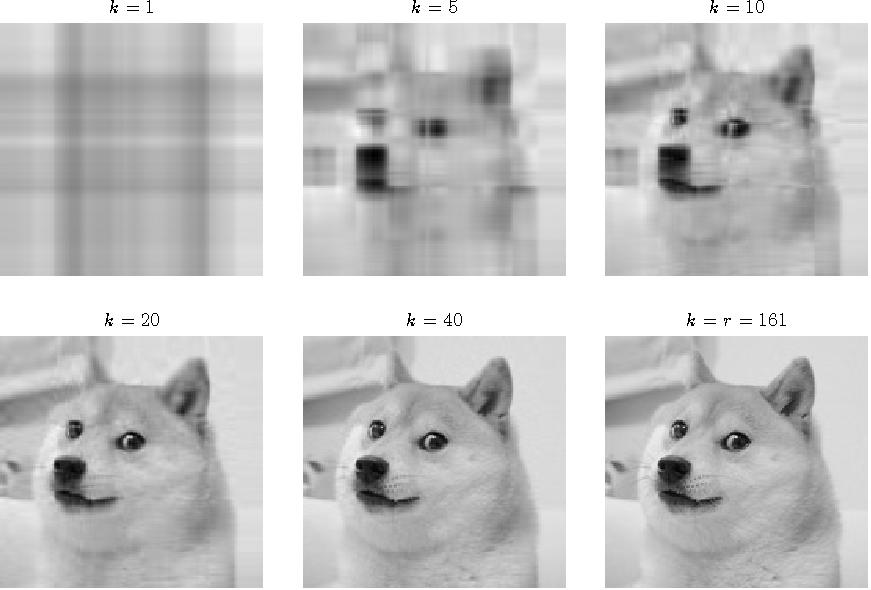
\includegraphics[width=0.8\linewidth]{graphs/svcompress.pdf}
        \captionof{figure}{基于奇异值分解的doge meme灰度图的压缩}
    \end{center}
\end{example}

\section{矩阵的模}

我们用内积定义了向量的模(即长度)
\[
	\norm x:=\sqrt{\inp xx}.
\]
下面我们用向量的范数诱导矩阵的范数。
\begin{theorem}{}{max Ax/x}
	\begin{equation}
		\norm{Ax}\leqslant\sigma_1\norm x.
	\end{equation}
\end{theorem}
\begin{proof}
	
	\begin{align*}
		\norm{Ax}^2&=x\tp A\tp Ax=x\tp V\Sigma\tp\Sigma V\tp x\\
		&=\sum_{k=1}^nx\tp v_k\sigma_k^2v_k\tp x\leqslant\sigma_1^2\sum_{k=1}^nx\tp v_kv_k\tp x\\
		&=\sigma_1^2x\tp VV\tp x=\sigma_1^2x\tp x,
	\end{align*}
	等号可在$x=cv_1$时成立。
\end{proof}
\begin{definition}{矩阵的模}{norm of matrix}
	矩阵的模(norm)定义为 
	\begin{equation}
		\norm A:=\max_{x\neq 0}\frac{\norm{Ax}}{\norm x}=\sigma_1.
	\end{equation}
\end{definition}
\begin{corollary}
	由矩阵模的定义可直接导出$\forall x\neq 0$,
	\[
		\norm{Ax}\leqslant\norm A\norm x.
	\]
\end{corollary}
\begin{theorem}{三角不等式}{triangle inequality}
	\begin{equation}
		\norm{A+B}\leqslant\norm A+\norm B.
	\end{equation}
\end{theorem}
\begin{proof}
	$\forall x\neq 0$,
	\[
		\norm{(A+B)x}=\norm{Ax+Bx}\leqslant\norm{Ax}+\norm{Bx}\leqslant\norm A\norm x+\norm B\norm x.
	\]
	故
	\[
		\norm{A+B}\leq\frac{\norm{(A+B)x}}{\norm x}\leqslant\norm A+\norm B.
	\]
\end{proof}

给定矩阵$A$,限定矩阵$B$的秩$\rank(B)=k<\rank(A)$,如何使得$B$最接近$A$?即
\[
	B^\star=\arg\min_B\norm{A-B}.
\]

\begin{theorem}{Eckart-Young-Mirsky定理}{Eckart-Young-Mirsky theorem}
	同矩阵$A$最接近的秩为$k$的矩阵为
	\begin{equation}
		A_k=\sum_{i=1}^k\sigma_iu_iv_i\tp.
	\end{equation}
\end{theorem}
\begin{proof}
	只需证$\forall B$秩为$k$,都有
	\[
		\norm{A-B}\geqslant\norm{A-A_k}=\sigma_{k+1}.
	\]
	设$w=c_1v_1+\cdots+c_{k+1}v_{k+1}$,因为$\rank(B)=k$,故$Bv_1,\ldots,Bv_{k+1}$必然线性相关,继而存在非零的$c_1,\ldots,c_{k+1}$使得$Bw=0$,在此基础上再归一化$w$,从而
	\begin{align*}
		\norm{A-B}^2&\geqslant\norm{(A-B)w}^2=\norm{Aw}^2\\
		&=\sigma_1^2c_1^2+\cdots+\sigma_{k+1}^2c_{k+1}^2\geqslant\sigma_{k+1}^2(c_1^2+\cdots+c_{k+1}^2)=\sigma_{k+1}^2.
		\qedhere
	\end{align*}
\end{proof}

\section{伪逆}

\begin{definition}{伪逆}{pseudoinverse}
	$m\times n$矩阵$A=U\Sigma V\tp$,定义伪逆(pseudoinverse)是一个$n\times m$的矩阵
	\begin{equation}
		A^+:=V\Sigma^+U\tp.
	\end{equation}
	其中$\Sigma^+$是一个$n\times m$的矩阵
	\[
		\Sigma^+:=\begin{bmatrix}
			D\iv&0\\0&0
		\end{bmatrix},\quad D\iv=\diag(\sigma_1\iv,\ldots,\sigma_r\iv).
	\]
\end{definition}

\begin{corollary}
	\begin{subequations}
		\begin{align}
			AA^+A&=A,\\
			A^+AA^+&=A^+.
		\end{align}
	\end{subequations}
\end{corollary}

\begin{remark}
	伪逆与原矩阵的乘积并不是单位矩阵:
	\[
		A^+A=V\begin{bmatrix}
			I_r&0\\0&0
		\end{bmatrix}V\tp,
	\]
	是投影到$\C(A\tp)$的矩阵;
	\[
		AA^+=U\begin{bmatrix}
			I_r&0\\0&0
		\end{bmatrix}U\tp,
	\]
	是投影到$\C(A)$的矩阵。
\end{remark}
\begin{theorem}{伪逆与最小二乘法}{}
	最小二乘法
	\[
		A\tp Ax=A\tp b,
	\]
	的解为$x^+=A^+b$。
\end{theorem}
\begin{proof}
	\[
		A\tp Ax^+=V\Sigma\tp U\tp U\Sigma V\tp V\Sigma^+U\tp b=V\Sigma\tp U\tp b=A\tp b.
		\qedhere
	\]
\end{proof}
\section{主成分分析}
一组数据$\mu=(\mu_1,\ldots,\mu_n)$来源于$n$个样本,其样本均值(mean)和样本方差(variance)分别为
\[
	\bar\mu=\frac1n\sum_{i=1}^n\mu_i,\quad\sigma^2=\frac1{n-1}\sum_{i=1}^n(\mu_i-\bar\mu)^2.
\]
将数据存在一个$m\times n$的矩阵$A$中,每一行对应一种数据,每一列代表一个样本。将每个元素减去其所在行的平均值
\[
	A_{ij}:=(A_0)_{ij}-\frac1n\sum_{k=1}^n(A_0)_{ik}.
\]
由此得到矩阵$A$,每一行都是以0为中心的分布。
\begin{definition}{协方差矩阵}{covariance matrix}
	定义协方差矩阵(covariance matrix)
	\begin{equation}
		S:=\frac{AA\tp}{n-1}.
	\end{equation}
	对角线上$S_{ii}$是样本方差;$S_{ij}$是样本协方差。
\end{definition}
\begin{method}{主成分分析}{principal component analysis}
	主成分分析(principal component analysis, PCA):找到原有数据的一系列线性组合作为新的数据,新数据之间的协方差为0.
\end{method}
利用$A=U\Sigma V\tp$,定义新的数据矩阵$B:=U\tp A=\Sigma V$,$B$的协方差矩阵
\[
	\frac{BB\tp}{n-1}=\frac{\Sigma\Sigma\tp}{n-1}
\]
是对角的,故$B$之间协方差为0。

总方差在这种变换下是不变的:
\[
	\tr\biggkh{\frac{BB\tp}{n-1}}=\frac{\tr(U\tp AA\tp U)}{n-1}=\frac{\tr(UU\tp AA\tp)}{n-1}=\tr\biggkh{\frac{AA\tp}{n-1}}.
\]
所有数据点分布在$\{u_1,\ldots,u_r\}$张成的$\C(A)$上,$u_1$是所有数据变化最大的方向(方差最大)、$u_2$次之……因此$\{u_1,\ldots,u_r\}$称作主成分(principal component)。
